REST(Representational State Transfer)という概念は2000年Roy Thomas Fielding(彼はHTTP仕様の主な著者の一人です。)の博士論文の中で初めて登場しました。この中ではあるフレームワークの制約条件と原則について触れています。これらの制約条件と原則を満足したアプリケーションまたは設計はRESTfulということです。

RESTが何かを理解するためには、以下のようないくつかの概念を理解する必要があります:

\begin{itemize}
  \item リソース(Resources)  RESTは"プレゼンテーション層の状態遷移"です。これは主語が省略されています。"プレゼンテーション層"というのは"リソース"の"プレゼンテーション層"です。
\end{itemize}

ではリソースとは何でしょうか?普段我々がアクセスする画像、ドキュメント、映像等です。これらのリソースはURIによって特定されます。つまりひとつのURIがひとつのリソースを表しています。


\begin{itemize}
  \item プレゼンテーション層(Representation)
\end{itemize}

リソースはある具体的な実体を伴う情報を作成します。これはいくつもの表現方法を持っており、実体の表現こそがプレゼンテーション層です。例えばtxtテキスト情報があれば、これはhtml、json、xml等の形式に出力することができます。画像はjpg、png等の方法で表現することができます。これがプレゼンテーション層の意味です。

 URIはひとつのリソースを確定します。しかしどのようにこの具体的な表現形式を確定するのでしょうか?HTTPリクエストのヘッダ情報においてAcceptとContent-Typeフィールドを用いて指定されているはずです。この2つのフィールドこそが"プレゼンテーション層"に対する描写なのです。


\begin{itemize}
  \item 状態遷移(State Transfer)
\end{itemize}

あるホームページにアクセスすることは、クライアントがサーバとインタラクティブな過程を表しています。この過程の中では必ずデータと状態遷移が関わってきます。HTTPプロトコルはステートレスですので、これらの状態はサーバに保存されているはずです。そのため、もしクライアントがサーバにデータの変更と状態遷移を通知したい場合は、なんらかの方法によってこれを通知する必要があります。

 クライアントがサーバに通知する手段はHTTPプロトコルしかありません。具体的にはHTTPプロトコルの中にある4つの操作方法を表す動詞:GET、POST、PUT、DELETEです。これらは4つの基本操作に分かれます:GETはリソースを取得するのに使われます。POSTはリソースを新規に作成するために使われます(リソースの更新に使うこともできます)。PUTは資源の更新に使われます。DELETEは資源の削除に使われます。

上の解釈を総合して、RESTfulフレームワークとは何かまとめてみます:

\begin{itemize}
  \item 各URIがひとつのリソースを表す
  \item クライアントとサーバ間で、これらの資源の何かしらのプレゼンテーション層を転送する
  \item クライアントは4つのHTTPの動詞を通して、サーバの資源に対し操作を行う。"プレゼンテーション層の状態遷移"の実現。
\end{itemize}

Webアプリケーションが満たすべきRESTの最も重要なルールは:クライアントとサーバ間のやりとりにおいてリクエスト間はステートレスだということです。すなわち、クライアントからサーバへの各リクエストはすべてリクエストが必要としている情報を含んでいなければなりません。もしサーバがリクエスト間のいかなる時点で再起動しても、クライアントはその通知を受けることができません。また、このリクエストはどのような利用できるサーバからによっても回答できます。これはクラウドコンピューティングといった環境に十分適しています。ステートレスですので、クライアントはデータをキャッシュすることで性能を改善することができます。

もうひとつ重要なRESTのルールはシステムの分離です。これはモジュールがこれと直接やりとりをしているレイヤのモジュールを除いて解除することができないことを示しています。システムの知りうる内容を単一のレイヤに制限することで、システム全体の複雑さを制限することができます。そのため、低レイヤの独立性を促すことができます。

下の図はRESTのフレームワーク図です:

\begin{figure}[H]
   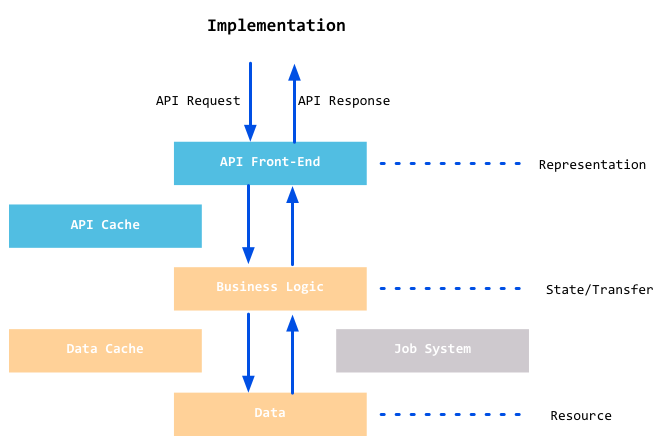
\includegraphics[width=14cm]{8.3.rest2.png}
   \label{図8.5}
   \caption{RESTフレームワーク図}
\end{figure}

RESTフレームワークの制約条件を全体に適用する際、大量のクライアントに向けて拡張できるアプリケーションプログラムを生成することができます。またクライアントとサーバ間のやり取りの遅延も減らします。統一されたインターフェースがシステムフレームワークの全体を簡略化し、サブシステム間のやり取りの見通しを改善します。RESTはクライアントとサーバの実装を簡略化し、RESTを使用して開発されたアプリケーションプログラムをより拡張しやすくします。

下はRESTの拡張性を示しています:


\begin{figure}[H]
   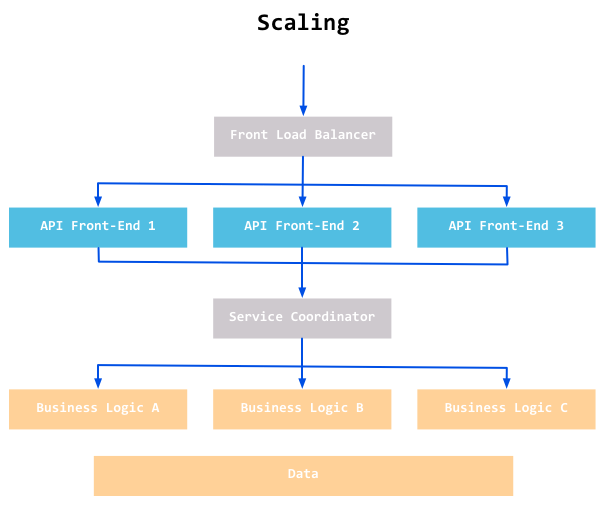
\includegraphics[width=14cm]{8.3.rest.png}
   \label{図8.6}
   \caption{RESTの拡張性}
\end{figure}





